\documentclass[a4paper,11pt]{book}
%% Language and font encodings
\usepackage[english]{babel}
\usepackage[utf8x]{inputenc}
\usepackage[T1]{fontenc}
%% Euro symbol
\usepackage{textcomp}

%% tabel rows
%% color rows table
\usepackage{xcolor}
\usepackage{color}
\usepackage{colortbl}
\definecolor{grayrow}{rgb}{0.85, 0.85, 0.85}
\definecolor{darkgrayrow}{rgb}{0.7, 0.7, 0.7}
\definecolor{RoyalRed}{rgb}{0.61,0.11,0.19}

%\usepackage{fancyhdr}
%\pagestyle{fancy}
%\fancyhf{}
%%\fancyhead[LE]{}
%\fancyhead[RE]{\rightmark}
%\fancyhead[LO]{\leftmark}
%\fancyhead[RO]{\thepage}
%\fancyfoot[CE]{\thepage}
%\renewcommand{\headrulewidth}{1pt} % it is too short!

%% chpater title style
% \usepackage[ ]{titlesec}  %
% \titleformat{\chapter}[display]
%   { \Huge \bfseries \rmfamily \color{black}}
%   {\flushright \color{RoyalRed} \bfseries \rmfamily \MakeUppercase { \chaptertitlename } \hspace{1 ex} { \fontsize{60}{60}\selectfont \bfseries \color{RoyalRed} \rmfamily \thechapter }} {15 pt}{\Huge}

\usepackage{emptypage} % remove header in blanck pages

%% Sets page size and margins
\usepackage[a4paper,top=3cm,bottom=2cm,left=3cm,right=3cm,marginparwidth=1.75cm]{geometry}

%% Useful packages
\usepackage{amsmath}
\usepackage{graphicx}
\usepackage{epigraph}
%\usepackage[colorinlistoftodos]{todonotes}
\usepackage[colorlinks=true, allcolors=blue]{hyperref}

% include file and not recompile it
\usepackage{standalone}

%% images directory
\graphicspath{{img/}}
%% colors
\hypersetup{
colorlinks,
citecolor=black,
filecolor=black,
linkcolor=black,
urlcolor=blue
}


\usepackage{listings}

\definecolor{codegreen}{rgb}{0,0.6,0}
\definecolor{codegray}{rgb}{0.5,0.5,0.5}
\definecolor{codepurple}{rgb}{0.58,0,0.82}
\definecolor{backcolour}{rgb}{0.95,0.95,0.92}

\lstdefinestyle{snippet}{
    backgroundcolor=\color{backcolour},
    commentstyle=\color{codegreen},
    keywordstyle=\color{magenta},
    numberstyle=\tiny\color{codegray},
    stringstyle=\color{codepurple},
    basicstyle=\ttfamily\footnotesize,
    breakatwhitespace=false,
    breaklines=true,
    captionpos=t,
    keepspaces=true,
    numbers=left,
    numbersep=5pt,
    showspaces=false,
    showstringspaces=false,
    showtabs=false,
    tabsize=2
}

\lstdefinestyle{c++}{
    backgroundcolor=\color{backcolour},
    commentstyle=\color{green}\ttfamily,
    keywordstyle=\color{blue}\ttfamily,
    numberstyle=\tiny\color{codegray},
    stringstyle=\color{red}\ttfamily,
    basicstyle=\ttfamily\footnotesize,
    morecomment=[l][\color{magenta}]{\#}
    breakatwhitespace=false,
    breaklines=true,
    captionpos=t,
    keepspaces=true,
    numbers=left,
    numbersep=5pt,
    showspaces=false,
    showstringspaces=false,
    showtabs=false,
    tabsize=2
}

\usepackage[]{algorithm2e}

%% Custom commands

\newcommand{\quotes}[1]{``#1''}

%% Start Document
\begin{document}

\documentclass{standalone}

\begin{document}

\begin{titlepage}

\centering

\includegraphics[scale=0.5]{unibo.png}

\begin{center}
{{\Large{\textsc{Alma Mater Studiorum $\cdot$ Universit\`a di Bologna}}}}
\rule[0.1cm]{15.8cm}{0.1mm}
\rule[0.5cm]{15.8cm}{0.6mm}
\\\vspace{3mm}

{\small{\bf Physics and Astronomy Department\\PhD Thesis in Applied Physics}}

\end{center}

\vspace{23mm}

\begin{center}\textcolor{black}{
{\Large{\bf Implementation and optimization of algorithms\\in Biological Big Data Analytics}}\\
}\end{center}

\vspace{40mm} \par \noindent

\begin{minipage}[t]{\textwidth}
{\large{\bf Supervisor: \vspace{2mm}\\\textcolor{black}{
Prof. Daniel Remondini}}}\\\\
{\large{\bf Correlator: \vspace{2mm}\\\textcolor{black}{
Prof. Gastone Castellani\\
Prof. Armando Bazzani}}}\\\\
\end{minipage}


\hfill

\begin{minipage}[t]{\textwidth}\raggedleft \textcolor{black}{
{\large{\bf Presented by:
\vspace{2mm}\\
Nico Curti}}}
\end{minipage}

\vspace{17mm}

\begin{center}
{\large{\bf Session \textcolor{black}{2019/2020}
}}
\end{center}

\end{titlepage}

\end{document}

\thispagestyle{empty}

\begin{flushright}
%% insert inscription (page 2)
\end{flushright}

%% Epigraph
\chapter*{}
\pagenumbering{gobble}% Remove page numbers (and reset to 1)
\epigraph{""\emph{No one know nothing,\\everyone know something,\\but something is nothing to someone,\\while\\something is important to everybody}''}{Daudi, Manyara}

%% Abstract
\pagenumbering{gobble}% Remove page numbers (and reset to 1)
\documentclass{standalone}

\begin{document}

\chapter*{Abstract}\addcontentsline{toc}{chapter}{Abstract}
\markboth{Abstract}{Abstract}

Every second a large quantity of data are produced and shared along Internet and Web-pages.
This is one of the main characteristic of our living time, the so-called Big Data era.


\end{document}


\tableofcontents
\newpage

%% Introduction

\pagenumbering{arabic}% Arabic page numbers (and reset to 1)
\documentclass{standalone}

\begin{document}

\chapter*{Introduction}\label{Introduction}\addcontentsline{toc}{chapter}{Introduction}
\markboth{Introduction}{Introduction}

Big Data: these two words are at the heart of many contemporary researches.
Nevertheless, it is yet a blanket term and no exhaustive description has been provided.
We commonly associate this term to the description of data generated from several machines and used to describe very complex system.
We can find Big Data associated to multiple kinds of modern researches which use this term to highlight the complexity of their projects.
The use of Big Data, in fact, is closely related to the Complexity term (intended with its physical meaning) and to the major part of Artificial Intelligence researches since they seem to be the only way to overcome these problems.
As anticipated, it is difficult to find a satisfactory definition about them and the common sense tends to identify them as simply a vast amount of data.
However, this is just a broadly description of them and it simplifies too much their usage and power.
We can find Big Data in more applications and fields than we usually think and a prominent research field is the Biomedical one.

Biomedical data are growing both in size and breath of possible uses.
This growth is driven by the development of newer and cheaper technologies for the acquisition of data which enlarge the availability of them.
At the same time, also the computational power is increasing and we can take advantage of more efficient and complex algorithms and pipelines for the analysis of a such amount of data.
Unfortunately, this second growth is not enough fast to tackle these problems and the development of novel techniques of processing and, moreover, algorithms able to extract informative portions of data is essential in the so-called Big Data Analytics.
This is even more true when we talk about Biomedical Big Data and thus data related to health-care studies which aim to identify the variable responsible for more or less complex diseases or to give a description of the more complex biological processes.
In addition to the novel \emph{Next Generation Sequencing} (NGS) technologies related to the analysis of biological structures like DNA and RNA, the so-called \emph{omics} researches involve a large part of contemporary biomedical researches.
The term \emph{omic} data, also in this case, refers to the wide range of biological studies ending in -omics, like \emph{genomics}, \emph{proteomics} or \emph{metabolomics} which aim to describe and quantify biological processes at different scale levels.
The analysis of these kinds of data poses many challenges to the research community, especially for the vast amount of variable involved.
For all we may work with Big Data, the biological research field is used to analyze only few samples compared to the number of variables involved: this is exactly the opposite behavior of common statistical analyses and, moreover, of physic research.
The ability to extract information and reduce the problem dimensionality is crucial to address these problems.

More complex analyses related to high dimensional problems are the image processing ones.
Biomedical imaging is another of the most prominent kind of analysis for the development of novel medical treatments.
The many differences between acquisition methods and data structures/characteristics for different imaging modalities create a zoo of possible studies and analyses.
At the same time, the dimensionality of the involved images requires an adequate computational effort.
These characteristics satisfy all the requirements pose by the modern deep learning training.
It is not always possible create an appropriated mathematical model to describe the underlying dataset and in many cases there is the need to handle more general applications.
Standard machine learning methods can not keep up such requirements and they are giving way to deep learning models.
In many applications these models are used as black-boxes and their complexity does not always allow a complete understanding about their learning.
Nevertheless, their efficiency is overcoming standard methods in a vast amount of applications and they are the only tools which provide the semblance of an artificial intelligence.

All these data and analyses involve multiple scientific researches which driven by them are becoming more accurate but, at the same time, also more specialized.
With a such heterogeneity of data, we can handle very useful analyses of any biological compound with a payback of a loss about the system complexity and interactions.
The absence of a standardized system for sharing biomedical information contributes to the difficulty about merging results provided by different studies.
Several European project about health-care research has been financed aiming to develop an harmonization between biomedical data sources.
The principal issues about this topic are related to a non rigid nomenclature of medical keywords and data formats.
Relational databases have efficiently driven Big Data research up to now, but the increasing demand of non-trivial connections between different kind of entries is paving the way to different kind of approaches and data management.
At the same time, also the research about novel natural language processing methods are becoming very popular in these applications.

This work of thesis started from these multiple issues about Big Data and it focus on different Biomedical topics.
In each chapter we are going to handle a different aspect of Big Data research and a different kind of data.
For each topic we provide a balanced description between the mathematical/theoretical background and numerical issues/solutions of it.
The main focus of each application remains its algorithmic description and the numerical solutions developed to handle the underlying problem.

We start our trip across Biomedical Big Data introducing a novel feature selection algorithm.
The proposed algorithm is tailored for gene expression analyses and in the various sections we provide a description of all its pros and cons.
The algorithm was already used in previous scientific publications but, for the first time, a deeper analysis of all its characteristics either from a numerical either from a algorithmic point-of-views is provided.
The algorithm has also undergone an intensive optimization procedure to make it able to handle Big Data problems in a reasonable computational time.
We firstly test our method against a custom toy model and only later we compare its efficiency against state-of-art equivalent models and data.
We also show some applications of it to different kind of data, starting from gene expression datasets, passing to protein expression levels until non-biological data proving its efficiency in all these topics.
Within the limits of our knowledge about biological process we provide also an interpretation about the obtained results where it is possible.

Then, we will move to more numerical expensive analyses with the help of modern deep learning models.
Starting from a brief introduction about neural network models we shall look at the different functions/layers included in the later discussed models.
For each of them we provide a theoretical explanation about the mathematical functions and, also in this case, we deeply focus on their numerical implementation.
Three custom libraries are introduced to help us in the description of these models and their results are discussed against other state-of-art implementations.
We use deep learning neural network models to handle different kind of image processing analyses with a particular attention to biomedical images.
As previous discussed, there are multiple image formats in the biomedical field and in our applications we use NMR and CT images.
Starting from modern Super Resolution algorithms we show their application on NMR image proving how they can help to increase the biomedical image quality and how they can be also used to improve object detection tasks.
Other kinds of applications are also shown to prove the versatility of such methods in several biomedical tasks.

We conclude our discussion introducing a novel database obtained by the harmonization of public available datasets.
A global description about Big Data sources and how we can handle problems related to the data extraction is discussed before our pipeline of processing.
A key role in our work is played by natural language processing methods and, thus, starting from a brief introduction about them we focus on the developed pipeline.
The work concerned the merging of multiple datasets into a unique network structure ables to manage the interactions between different biomedical compounds.
The network-of-networks structure generated during this project allows a wider overview of several diseases pointing out their association to genes, drugs and other biological data.
We also discuss about how this large amount of information can be managed using modern database languages and about the chosen strategy to share our results to the scientific community.

For sake of brevity, not all the developed projects are discussed and some of the remaining ones are bounded in the Appendix of this text.
However, the principal contributions of this work are related to the developed codes.
All the code described in this work are, in fact, public available on-line on Github (\url{https://github.com/Nico-Curti/}).
We have paid special attention to the development of our codes, carefully managing their testing and availability.
Each code has been enriched by an adequate on-line documentation either about its usage either about its installation and performances.
A small part of the codes have been written in pure-\textsf{Python} while the major part has been written in \textsf{C++}: for this reason a continuous integration of them is essential to ensure their usability.
We remark that also the current text is public available on Github as \textsf{Latex} code and to facilitate its reading and its hyper-link connections we have converted it also into a \textsf{Gitbook} version available at \url{https://nico-curti2.gitbook.io/phd-thesis/}.


% take something from the EuroPar18 introduction

% in questo lavoro si affronteranno diverse tematiche relative alla Big Data Analytics e si propongono soluzioni inerenti ad ognuna di esse con esempi sviluppati ed applicati a dati reali.
% Partendo dalla curse of dimensionality e la feature extraction (dnet), passando per la visualizzazione dei dati con le NN fino alla eterogeneità dei dati (chimera)

% definire feature come variable e dire che nel resto del testo verranno usati in maniera indistinta i due termini

\end{document}


%% Chapter 1 - DNetPRO algorithm

\documentclass{standalone}

\begin{document}

\chapter[Feature Selection]{Feature Selection - DNetPRO algorithm}\label{featsel}

Introduction to feature selection problem and theoretical background.

Focus on biological Big Data and problems related.


\end{document}

% Introduction to feature selection problem and theoretical background. Focus on biological Big Data and problems related.

\documentclass{standalone}

\begin{document}

\section[DNetPRO algorithm]{DNetPRO algorithm}\label{DNetPRO}

The DNetPRO algorithm generates multivariate signatures starting from all couples of variables tested with Discriminant Analysis.
For this reason it can be classified as a combinatorial method and the computational time for variable space exploration is proportional to the square of the number of available variables (ranging from $10^3$ to $10^5$ in a typical high-throughput omics study).
This behavior allows it to overcome some of the limits of single-feature selection methods, and provides a hard-thresholding approach at difference with projection-based variable selection methods.
Certainly the combination evaluation is the most time expensive step of the algorithm and it needs accurate algorithmic implementation for Big Data applications (see the next section for further informations about the algorithm implementation strategy).
The algorithm can be summarize as shown in~\ref{code:DNetPRO}.

\begin{algorithm}[H]
  \KwData{Data matrix (N, S)}
  \KwResult{List of putative signatures}
  Divide the data into training and test by an Hold-Out method\;
  \For{$couple$ $\leftarrow$ ($feature\_1$, $feature\_2$) $\in$ $Couples$}{
    Leave-One-Out cross validation\;
    Score estimation using a Classifier\;
  }
  Sorting of the couples in ascending order according to their score\;
  Threshold over the couples score ($K$best couples)\;
  \For{$component$ $\in$ $connected\_components$}{
    \eIf{$reduction$}{
      Iteratively pendant node remotion\;
    }
    Signature evaluation using a Classifier\;
  }
  \caption{DNetPRO algorithm for Feature Selection.}
  \label{code:DNetPRO}
\end{algorithm}

So, given an initial dataset, consisting in $S$ \emph{samples} (e.g. cells or patients) with $N$ observations each (our \emph{variables}, e.g. gene or protein expression profiles), the signature identification procedure can be summarized with the following pipeline:

\begin{itemize}

\item separation of available data into a training and a test set (e.g. 33/66, or 20/80);

\item estimation of the classification performance on the training set of all $S(S-1)/2$ variable couples through a computationally fast and reproducible cross-validation procedure (leave-one-out cross validation was chosen);

\item selection of top-performing couples through a hard-thresholding procedure.
The performance of each couple constitutes a \emph{weighted link} of a network in which nodes are the variables connected at least through one link;

\item every \emph{connected component} in which the network is divided into constitutes an identified classification signature.

\item (optional) in order to reduce the size of an identified signature, the pendant nodes of the network (i.e. nodes with degree equal to one) can be removed, in a single step or recursively until the core network (i.e. a network with all nodes with at least two links) is reached.

\item all signatures are applied onto the test set to estimate their performance.

\item a further cross validation step is performed (with a further dataset splitting into test and validation sets) to identify the best performing signature.

\end{itemize}

I would stress that this method is completely independent to the chose of the classification algorithm but from a biological point of view a simple one is preferred to preserve an easy interpretability of the results.
The geometrical simplicity of the resulting class-separation surfaces, in fact, allows an easier interpretation of the results, as compared with very powerful but black-box methods like nonlinear-kernel SVM or Neural Networks.
Moreover the network interaction of variables can keep an internal ranking score of features importance or possible features cooperation.
These are the reasons that move us to use very simple classifier methods in our biological application as diag-quadratic Discriminant Analysis or Quadratic Discriminant Analysis (Appendix A for more informations about the mathematical background and implementation in the different languages).
Both these methods allow fast computation and easy interpretation of the results.
This linear separation might not be common in some classification problems (e.g. image classification) but it is very plausible in biological systems, in which many responses to perturbation consist in increase or decrease of variable values (e.g. expression of genes or proteins, see Fig.~\ref{fig:example}(b)).

In a general classification problem (e.g. image analysis) this could not be the case, since complex non linear separating surfaces may exist among the classes, but we hypothesize (and our results seem to confirm so) that in classification problems based on biological data such as gene expression these situations are not so common.
This assumption is very plausible for biological data, since genes are in general up- or down-regulated in order to modify their activity, and protein and metabolites most of the times respond consequently.

A second direct gain by the couples evaluation is related to the network structure: the DNetPRO network signatures allow a hierarchical ranking of the features according to their centrality compared to possible Kbest signatures.
This underlying network structure of the signature could suggest further methods for signature dimensionality reduction based on network topological properties to fit real application needs and it could help to evaluate the cooperation of the variables for the class identification.





\section[Toy Model]{Synthetic dataset benchmark}\label{toy}

We firstly tested the DNetPRO method with synthetic data, consisting in a small set of discriminating variables together with a large number of \quotes{noisy} variables.
Fixing the number of informative features and classes we test the DNetPRO efficiency on the features extraction, compared to the results obtained by individually single features ranking (\emph{Kbest} feature selection).

To simulate a synthetic \quotes{gene expression dataset}, with a large number of variables and a much smaller number of samples, we use the toy \href{https://scikit-learn.org/stable/modules/generated/sklearn.datasets.make_classification.html}{model generator} provided by the \emph{scikit-learn}~\cite{scikit-learn} python package.
This model generator allows to set a precise number of classes and it distinguishes between \emph{informative features}, i.e. features which easily separate the class populations, and \emph{redundant features}, i.e. features which represent noise in our problem.
The number of informative features should be realistically small compared to the noise, so in our simulations we chose to introduce at least a 10\% of informative features in the whole dataset.

% TODO: simulations and results

%Method description.
%Efficiency on a biological toy model.



\end{document}

% Description of the method and efficiency a biological toy model.

\documentclass{standalone}

\begin{document}

\section[DNetPRO Implementation]{Algorithm implementation}\label{implementation}

Description of the algorithm implementation in C++.
Parallelization of the algorihtm.
Use of BGL for network processing (filter node using view)
Wrap in Python for Sklearn use
Time Performances on different machines.


\end{document}
% Description of the algorithm implementation with focus on performances of the new implementation.

\documentclass{standalone}

\begin{document}

\section[Synapse Dataset]{Synapse dataset}\label{synapse}

Description of the synapse datasets.
Application of the DNetPRO on the Synapse dataset (mRNA, miRNA, RPPA) of Yuan et al. with two different pipelines.
Discussion on obtained performances compared to the most common machine learning methods.
Discussion on the ranking.
Discussion on the extracted signature.



\end{document}
% Application of the DNetPRO on the Synapse dataset (mRNA, miRNA, RPPA) of Yuan et al. with discussion about obtained performances compared with the most common ML methods and signature characterization

\documentclass{standalone}

\begin{document}

\section[Cytokinoma Dataset]{Cytokinoma dataset}\label{cytokine}

Description of the cytokinoma dataset with statistics.
Application of the DNetPRO on the Cytokine dataset.
Discussion on the obtained signature and biological interpretation of the Alzheimer disease.


\end{document}
% Application of the DNetPRO on the Cytokine dataset with data description and obtained results

\documentclass{standalone}

\begin{document}

\section[Bovine Dataset]{Bovine Paratuberculosis}\label{bovine}

Paratuberculosis or Johne's disease (JD) in cattle is a chronic granulomatous gastroenteritis caused by infection with \emph{Mycobacterium avium subspecies paratuberculosis} (MAP).
JD is not treatable; therefore the early identification and isolation of infected animals is a key point to reduce its incidence worldwide.
In this work DNetPRO algorithm was applied to RNAseq experimental data of 5 cattle positive to MAP infection compared to 5 negative uninfected controls.
The purpose was to find a small set of differentially expressed genes able to discriminate between infected animals in a pre-clinical phase.
Results of the DNetPRO algorithm identified a small set of 10 transcripts that differentiate between potentially infected, but clinically healthy, animals belonging to paratuberculosis positive herds and negative unexposed animals.
Furthermore, the same set of 10 transcripts differentiate negative unexposed animals from positive animals based on the results of the ELISA test\footnote{
  The enzyme-linked immunosorbent assay.
  It is a common diagnostic tool as well as a quality control check in various bio-medical industries and in medicine.
} for bovine paratuberculosis and fecal culture.
Within the 10 transcripts that together had good discriminative potential, 5 (TRPV4, RIC8B, IL5RA, ERF and CDC40) show significant differential expression between the three groups while the remaining 5 transcripts (RDM1, EPHX1, STAU1, TLE1, ASB8) did not show a significant differences in at least one of the pairwise comparisons.
In conclusion, the discriminant analysis described here identified a set of 10 genes that discriminate between the exposed and sero-converted animals.
When tested in a larger cohort, these finding lead the possible use of RNA expression analysis as new diagnostic test for paratuberculosis.
Such a signature could allow early interventions to reduce the sanitary and economic burden, and to reduce the risk of infection spreading.

In the next sections a description of the dataset and of main DNetPRO results will be discussed.
Further informations can found in the original paper~\cite{Malvisi2019}.

\subsection[Dataset]{Dataset}\label{bovine_data}

Paratuberculosis or Johne's disease (JD) in cattle is a chronic granulomatous gastroenteritis caused by infection with \emph{Mycobacterium avium subspecies paratuberculosis} (MAP).
JD is present worldwide, is a welfare issue and causes significant economic losses.
Cattle are usually infected as young calves but typically do not show clinical signs before 24 months of age, however not all infected animals progress to clinical disease.
JD is not treatable, therefore the early identification and isolation of infected animals, before they start shedding the bacteria, is a key point to reduce its incidence in cattle herds worldwide.
In addition, an association between MAP and Crohn's disease (CD) in humans has been suggested and intensively explored.
Given the economic losses and welfare concerns for livestock, and possible human health risk, the research interest in JD has been driven by the substantial difficulty in early diagnosis of infected animals and the exploration of potentially new diagnostic techniques.

The dataset used in this work was previously discussed and generated by some of the authors of the original paper.
In detail, the dataset used comprised 15036 transcripts from 15 samples, classified as \quotes{serologically negative non exposed cows/healthy} (5 samples, labeled as NN), \quotes{serologically negative exposed cows/ infected} (5 samples, NP) and \quotes{serologically positive cows/clinical} (5 samples, PP).
Only transcripts with non-zero measures for all samples were considered, reducing the dataset to 13529 transcripts.

All data generated or analyzed during this study is available upon request, furthermore all transcript counts per sample are given as supplementary information files of the original paper.



\subsection[Results]{Bovine Signature}\label{bovine_result}

In the context of high-throughput data analysis, a challenge is the search for an optimal choice of variables (a \quotes{signature}) to classify groups of samples or regress trends with optimal performance and minimum dimensionality.
Usually high-throughput omics data (e.g. transcriptomics, ge-nomics, methylomics) provide datasets with few tens to hundreds of samples, and often 1000 times larger numbers of variables.
The objective of dimensionality reduction through the choice of an optimal signature is twofold: 1) the identification of relevant variables, that should separate the signal from the noise (i.e. variables not significantly associated to, or descriptive of the studied process); 2) in a practical context, it is important to establish future diagnostic criteria that can be implemented in cheap and simple toolkits, such as PCR cards or dedicated microarray chips, that usually test a small number of transcripts (ranging from tens to hundreds, at most).
The quantity of samples compared to the available features of this work, join with the final purposes of this kind of analysis, set the well-known ill-posed problem conditions for which the DNetPRO algorithm was thought.

Since the number of sample is drastically small no robust cross-validation procedure can be applied.
So we focused on the identification of a putative gene-signature able to discriminate between NN and NP samples, leaving the PP data as validation set.
In this case we hypothesize that PP samples will be classified more closely with NP sample rather than NN as exposed, possibly infected samples, should be more similar to positive samples, than to negative controls.

\begin{figure}[htbp]
\centering
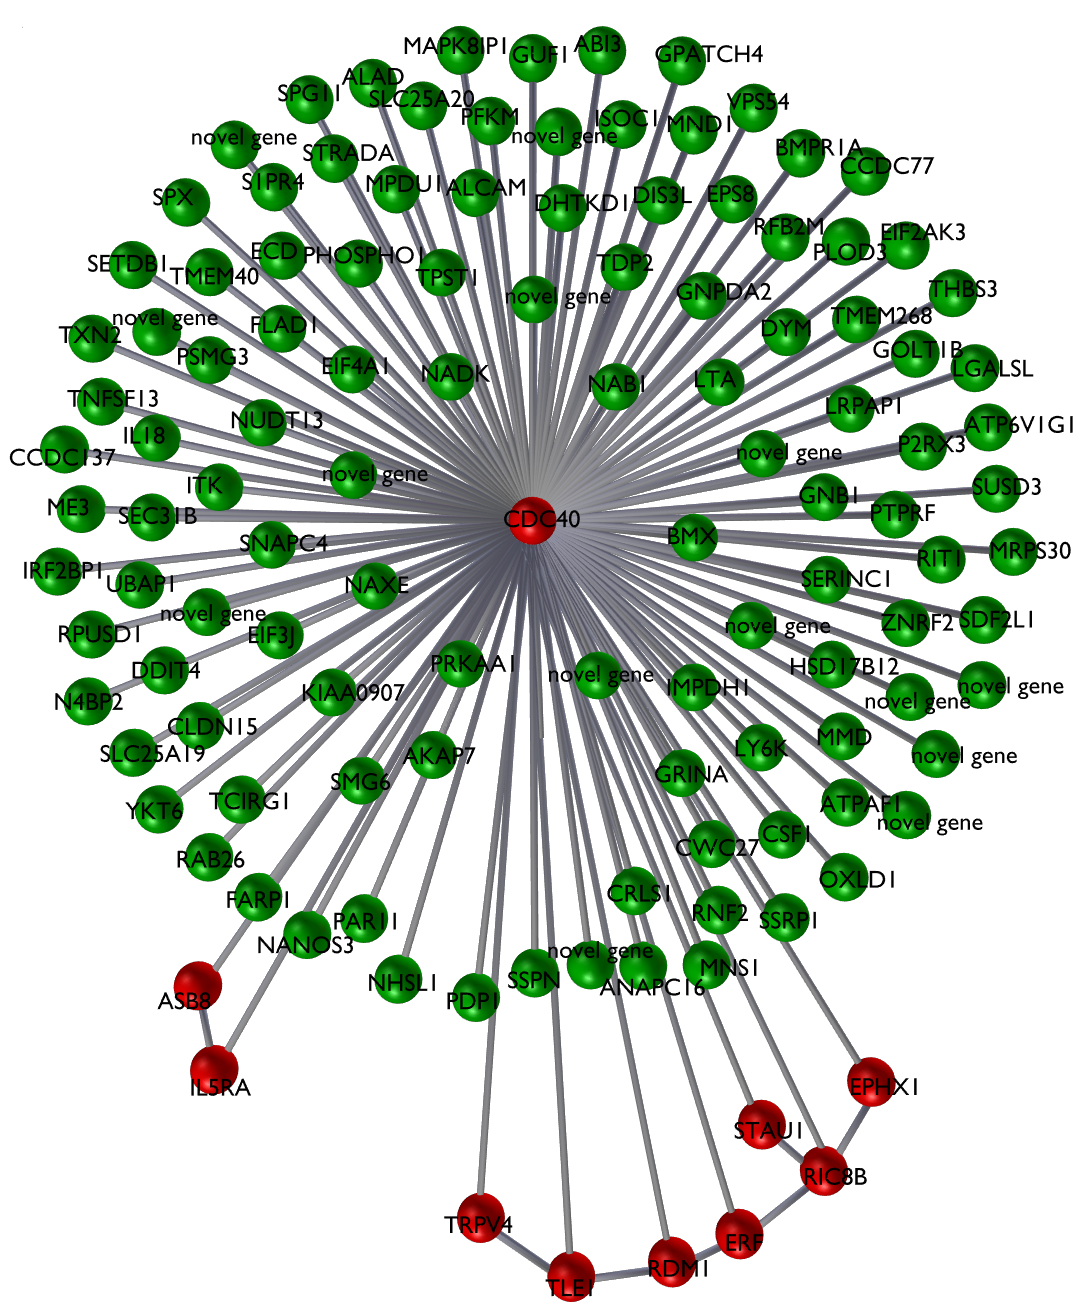
\includegraphics[width=0.4\textwidth]{./img/Bovine_signature.png}
\qquad\qquad
\def\svgwidth{0.45\textwidth}
\input{./img/Bovine_expression_level.pdf_tex}
\caption[Caption Bovine]{(\textbf{a}) Plot of the 123-transcript network, with a details of the 10-probe signature (red nodes)\footnotemark.
(\textbf{b}) Transcript levels for the 10 genes belonging to the classification signature identified by the combinatorial discriminant analysis (CDA).
Some transcripts (EPHX1, RIC8B, IL5RA, ERF, CDC40) show a clear trend  between 5 animals serologically positive to the ELISA test for MAP (PP), 5 exposed serologically negative (NP) and 5 serologically negative unexposed control animals (NN).
}
\label{fig:bovine_signature}
\end{figure}
\footnotetext{
  The figure was generated using a custom network visualizer described in Appendix C - BlendNet.
}


Starting from the top-performing couples of transcripts, we obtained an initial signature of 123 different transcripts (Fig~\ref{fig:bovine_signature}(a), all the nodes), capable to correctly classify 4 out of the 5 NN samples (80\%) and all 5 NP samples (100\% performance).
The average performance was therefore 90\% with Matthews correlation coefficient MCC = 0.82.
Processing the 123-transcript network by removing all pendant nodes (i.e. removing all single transcripts belonging to only one best-performing couple) we obtained a final signature with 10 transcripts with a 100\% performance classifying all NN and NP samples (Fig~\ref{fig:bovine_signature}(a), only red nodes).
As it can be seen, many nodes are directly connected to the central node (belonging to the 10-transcript signature), while only the 10 transcripts of the signature are also connected between each other.

Principal Component Analysis of the 10-transcript signature showed that in many cases there was a progressive increase or decrease in the transcript levels when passing from a healthy (NN) sample to a positive (PP) sample, passing through the infected (NP) sample class.
Fig~\ref{fig:bovine_signature}(b) shows the expression levels of the transcripts belonging to the signature for all samples.

To further validate the goodness of the signature, we generated 10000 different signatures with 10 randomly chosen transcripts, and then applied a Leave-One-Out cross validation procedure to classify all 15 samples with these signatures.
Comparing the performance of the random signatures with the true 10-transcript signature, only 50 of these signatures (corresponding to 0.5\% of the random signature distribution) produced better performance than our signature in terms of classification performance, confirming its high significance.

We even characterized the possible biological role of the signature genes, among the significantly differentially expressed genes, the cell division cycle 40 gene (CDC40) showed the smallest fold change between classes.
However in the identified signature the CDC40 gene is the most central node associated with the health status of the animals related to JD.
CDC40 was also under expressed in the NP and PP groups, compared with the NN group and it has been shown to be involved in clathrin medated endcytosis from a biological point-of-view.
Clathrin is the best characterized coat protein involved in the endocytosis process, specifically in receptor-mediated-internalization.
\emph{Mycobacterium paratuberculosis} enters the host macrophages, its primary target cell, and manages to survive within their phagosome.
It is possible that the under-expression of CDC40 in infected and sick animals compared to unexposed animals may be associate with down regulation of macrophage genes post mycobacterial invasion, facilitating the survival of the pathogen with the host target cell.

Interestingly within the set of 10 discriminating transcripts, in addition to CDC40, others show links with immune response mechanisms, these include IL5RA, ERF and TRPV4.
These genes potentially have functions related to the biology of progression of JD.
Also for the other genes of the final 10-transcript signature a possible biological interpretation related to JD was given (see the original paper for further descriptions).

In conclusion, the DNetPRO algorithm identified a set of 10 genes, the expression levels of which could discriminate between the exposed and sero-converted animals.
These finding lead the possible use of RNA expression analysis as new diagnostic test for JD.
In particular the approach may be able to identify infected animals prior to sero-conversion, prior to a positive ELISA test result.
However, further tests for specificity and validation in a larger cohort are required.


%Description of the bovine dataset with biological background.
%Application of the DNetPRO on the Bovine dataset with the description of the two singatures extracted.
%Discussion on biological interpretation of the genes.

% cite and describe BlendNet repo in the signature figure

\end{document}
% Application of the DNetPRO on the Bovini dataset with data description and obtained results with biological interpretation


%% Chapter 2 - Neural Network and Byron

\documentclass{standalone}

\begin{document}

\chapter[Deep Learning]{Deep Learning - Neural Network algorithms}\label{neural}

Description of the modern deep neural networks.
Computational problems and potential applications


\end{document}

% Description of the modern deep neural networks with potential applications

\documentclass{standalone}

\begin{document}

\section[NumPyNet]{Neural Network laboratory - NumPyNet}\label{numpynet}

%Description of the Neural Network laboratory developed in pure numpy.
%Study of the neural network functionality.
%Testing of the code against tensorflow.



\end{document}

% Neural Network laboratory developed in pure numpy. Study of the neural network functionality and testing of the code against tensorflow

\documentclass{standalone}

\begin{document}

\section[rFBP]{Replicated Focusing Belief Propagation}\label{rfbp}

Description of the rFBP library as optimization of the Julia code.
Pure c++ implementation with Python wrap (sklearn compatibility).
Scorer library as performance evaluation tool with parallel evaluation of scorers.

\end{document}

% rFBP library to optimize the Julia code with reference to the Scorer library and application to COMPARE data (Daniele Thesis)

\documentclass{standalone}

\begin{document}

\section[Byron]{Build YouR Own Neural network - Byron library}\label{byron}

Limits of the most common neural network frameworks.
Neural Network library for parallel computing developed in C++.
Pyron as python wrap of the library.
Description of the algorithms used to optimize the computation (ex. im2col vs winograd).


\end{document}

% Neural Network library for parallel computing developed in C++ with python wrap. Description of the algorithms and strategies chosen in the library development.

\documentclass{standalone}

\begin{document}

\section[Yolo]{Object Detection - Yolo architecture}\label{yolo}

%Introduction on the image classification and detection with Yolo architecture.
%Implementation in Byron with description of performances against darknet (original implementation).
%Focus on performances (time, memory, cpu).


\end{document}

% Introduction on the image classification and detection with Yolo architecture. Implementation in Byron with description of performances against darknet (original implementation). Focus on performances (time, memory, cpu).

\documentclass{standalone}

\begin{document}

\section[WDSR]{Super Resolution - WDSR architecture}\label{sr}

Introduction on Super Resolution problem with focus on state-of-art neural network architecture.
Description of the Byron implementation and application on NMR data with the most common measurements.
Super-resolution allows better detection!


\end{document}

% Introduction on Super Resolution problem with focus on state-of-art neural network architecture. Description of the Byron implementation and application on NMR data with the most common measurements. Super-resolution allows better detection!

\documentclass{standalone}

\begin{document}

\section[UNet]{Image Segmentation - UNet architecture}\label{unet}

%Introduction on Image Segmentation problem.
%Creation of the datasets with common image-processing methods % TODO: apply to the full set of the images
%Application of Unet (Byron implementation) on femur images. % TODO: all


\end{document}
 % OR rFBP
% Introduction on Image Segmentation problem and application of Unet (Byron implementation) on femur images (TODO)


%% Chapter 3 - CHIMeRA project

\documentclass{standalone}

\begin{document}

\chapter[Big Data]{Biological Big Data - CHIMeRA project}\label{bigdata}

Many public datasets available.
Description of the database used in chimera.
Problems about the intersections and partial informations (single db).


\end{document}

% Many public datasets available. Description of the database used in chimera

\documentclass{standalone}

\begin{document}

\section[Web Scraping]{Data extraction - Web scraping}\label{scraping}

Description of the web scraping techinques used to obtain the "no-public" datasets.
Reference to the github project.


\end{document}
% Description of the web scraping techinques used to obtain the "no-public" datasets. Reference to the github project

\documentclass{standalone}

\begin{document}

\section[CHIMeRA]{The CHIMeRA project}\label{chimera}

%What is CHIMeRA project and which is its potentiality.
%Description of the database created and of the query implemented to obtain the results %TODO: better query


\end{document}
% What is CHIMeRA project and which potentiality it has. Description of the database created and of the query implemented to obtain the results (TODO: better query)

\documentclass{standalone}

\begin{document}

\section[CHIMeRA query]{CHIMeRA query}\label{query}

%Some query examples like leukemia subnetwork and PRNP subnetwork.
%Description of the information extracted by these subnetworks. % TODO

\end{document}
% Some query examples like leukemia subnetwork and PRNP subnetwork. Description of the information extracted by these subnetworks


%% Chapter 4 - cardiological data

% \input{./tex/Chapter4/AppitechData.tex}
% % Description of the pulsoximmetry and of the cardiological data analyzed

% \input{./tex/Chapter4/CardioFeature.tex}
% % Description of the features extracted on the cardiological dataset

% \input{./tex/Chapter4/AgePrediction.tex}
% % Pipeline of the feature selection with age prediction obtained on cardio data

%% Conclusion

\documentclass{standalone}

\begin{document}

\chapter*{Conclusions}\label{conclusions}\addcontentsline{toc}{chapter}{Conclusions}
\markboth{Conclusions}{Conclusions}

We have concluded our discussion about the applications of Big Data Analytic algorithms to Biomedical data.
In this work we have touched several and different topics related to this theme.

In the first chapter we have focused on the difficulties about information extraction, analyzing high-throughput datasets.
The so-called \emph{omics} datasets are becoming a very interesting research field in biology and medicine since, using modern data acquisition techniques, they are capable to give a wide range of useful data for the analysis of multiple diseases.
A crucial role on this topic is given by tumors and, using \emph{omic} data, we can design novel methods to identify the agents responsible for these diseases.
Biomedical Big Data pose new challenges to the scientific research, since we have to convert them into useful information or, in other words, we have to be able to identify their informative cores.
To this purpose we have designed the new \textsf{DNetPRO} algorithm as a novel feature selection method.

We have tried to show all the pros and cons about the proposed algorithm.
Only knowing its limits we could be able to provide a reasonable interpretation about its results and for this reason we firstly tested our method on synthetic data.
The proposed \textsf{DNetPRO} pipeline was tailored on gene expression applications and we have shown its application on real data, comparing its efficiency against other state-of-art models in which it is able to outperform them in the major part of the analyzed cases.
Some these results are already published in international papers or they are in press.
We would remark that \textsf{DNetPRO} could be used also as standalone feature selection algorithm, but, for sake of brevity, we have discussed its application on non-biological data only in the Appendices of this work.

In the second chapter we have moved to numerical applications in the deep learning research field.
We have paid particular attention to the description and optimization of some state-of-art deep learning models.
In this chapter we have also introduced three new custom libraries about this topic, which have been developed with different purposes: the \textsf{NumPyNet} is essentially an educational framework for the development of neural network models, while the \textsf{Byron} library is focused on the numerical performances; the \textsf{rFBP} library was designed for very particular applications and in this work we have just briefly shown one of them.
Starting from the bases of neural network models, we have discussed about different kinds of functions (more or less straightforward) which are commonly involved in the construction of a deep learning neural network architecture.
For each function, we have only summarily described its mathematical background, focusing instead on the critical points related to its algorithmic implementation.

We have used the two developed libraries (\textsf{NumPyNet} and \textsf{Byron}) to highlight possible ways to overcome these numerical issues.
For sake of brevity, it has not been possible to go in deeper details about the numerical improvements performed, but all the developed codes have been shared and they are publicly available on the author's Github page.
The modern scientific research, in fact, is not made only by papers and publications but it is acquiring even more importance the code development and, thus, its public availability.
By sharing our code on the Internet, we want to encourage the research community to take in consideration also our promising results about these topics.
We have touched different state-of-art models and implementations of them along our discussion and in all the analyzed cases our results overcome them with not negligible results.

The results obtained using Super Resolution and Segmentation models are very promising for the analysis of biomedical images.
Moreover, we have shown that deep learning models are capable of a very efficient generalization due to their vast amount of parameters and a well-programmed training section.
In particular, our Super Resolution models were trained on general-purpose (natural) images, but they are, however, able to reconstruct biomedical NMR images better than standard methods.
This, already discussed, result is due to the ability of the model in the identification of analogous textures and patterns between the training and validation images, without need of a tailored retrain.
We have also seen how we can improve object detection efficiency using a pre - Super Resolution - processing: we could not show biomedical results on this topic due to lack of data and privacy reasons, but we have shown how a people-counting problem (Complex System task) is improved by this.

We would remark that our work was focused on the optimization of those codes only for CPU usages and, thus, we can not compare them to the wide world of GPU deep learning models.
We would, however, stress that we have intentionally chosen to focus only on these computational environments, aiming to increase the usage of this kind of models also in research fields which do not need GPUs in their everyday works.
There are, in fact, a lot of scientific applications which are tailored on CPUs architectures and which are pushed out to the deep learning researches, or which do not even try to use deep learning models afraid by their intensive computational demand.
We developed the \textsf{Byron} library to overcome these issues and to highlight how a well-thought-out algorithmic implementation can overcome also the more computational expensive applications.

All the developed algorithms were intensively profiled against other state-of-art implementations and their pros and cons have been examined in order to find the best solution for a given problem.
Code testing has been performed also on different operative systems, since how well an algorithm is made, it is useless if it works only on a well-defined machine.
A continuous integration of our codes has been at the basis of all the proposed libraries, as much as a reliable and user-friendly code documentation.

We have concluded our discussion introducing the \textsf{CHIMeRA} project which, even though the analysis of its results is still in work in progress, gives us multiple points of discussion about Biomedical Big Data.
There is an increasing interest about database harmonization in the last years and its need is given by the growing amount of publicly available data.
The research community is still trying to keep up with the new demand of data analysis and an increasingly important role is played by the development of new computational strategies and techniques.
Many European projects financed by the Horizon 2020 Research and Innovation program are focused on this topic and a particular attention is paid on the health-care research.

The \textsf{CHIMeRA} project could not be compared to such big research programs, but it is driven by the same kind of ideas.
Its final purpose, in fact, is to use the wide range of available information and results, obtained by independent research studies, and combine them into a unique framework of analysis.
Observational databases differ in both purposes and designs: they have been collected for different purposes and the logical organizations as much the medical terminologies can vary from source to source.
A \emph{Common Data model} (CDM) is designed to overcome these issues and to offer a unique solution for the information storage in the same way as our \textsf{CHIMeRA} project merges together information provided by multiple on-line databases.
Unfortunately, the research community is developing a wide range of CDMs and as long as a single solution is not taken as standard, the problem can not be solved.
Also in this case, we have not developed \textsf{CHIMeRA} as putative alternative to this purpose, but it is simply a temporary solution which allows us to perform a panoramic overview of biomedical agents.

We have highlighted multiple possible usages of the developed \textsf{CHIMeRA} network-of-networks structure and we hope it can be useful as an integrative tool also for the biggest projects like the HARMONY one.
In this work we have focused on the key steps which lead us to the ideas behind the \textsf{CHIMeRA} project and, moreover, we have described difficulties and their relative proposed solutions about the creation of a such network-of-networks database.
Despite the work has been intense up to now, the more interesting part from a scientific point-of-view is just began.
The \textsf{CHIMeRA} database is the only \quotes{code} discussed in this work which is not yet publicly available, due to its embryonic stage, but hopefully we can provide its first release as soon as possible.


\end{document}


%% Appendix

\documentclass{standalone}

\begin{document}

\chapter*{Appendix A - Discriminant Analysis}

The classification problems aim to associate a set of \emph{pattern} to one or more \emph{classes}.
With \emph{pattern} we identify a multidimensional array of data labeled by a pre-determined tag.
In this case we talk about \emph{supervised learning}, i.e the full set of data is already annotated and we have prior knowledge about data association to the belonging classes.
Since in this work only supervised learning algorithms have been analyzed we do not cite other different learning methods.

In machine learning a key rule is assumed by Bayesian methods, i.e methods which use a Bayesian statistical approach to the analysis of data distributions.
It can be proof that if the distributions under analysis are known, i.e a sufficient number of moments of it is known with a sufficient precision, the Bayesian approach is the best possible method to face on the classification problem. % cite!





\section*{Mathematical formulation}

Since the exact knowledge of the prior probabilities and conditional probabilities is possible only on theory a parametric approach is often needed.
A parametric approach aim to create reasonable hypothesis about the distribution under analysis and its fundamental parameters (e.g mean and variance).
In the next of this discussion we focused only on normal distributions for convenience.

Given the multi-dimensional form of Gauss distribution:

$$
G(\mathbf{x}|\mu, \Sigma) = \frac{1}{(2\pi)^{d/2}\cdot\left|\Sigma\right|^{1/2}}\cdot exp\left[-\frac{1}{2}(\mathbf{x}-\mathbf{\mu})^T\Sigma^{-1}(\mathbf{x}-\mathbf{\mu})\right]
$$
\\
where $\mathbf{x}$ is a column $d$-dimensional vector, $\mathbf{\mu}$ the mean vector of the distribution, $\Sigma$ the covariance matrix ($d\times d$), $|\Sigma|$ and $\Sigma^{-1}$ the determinant and the inverse of $\Sigma$, respectively, we can notice the $G$ depends quadratically by $\mathbf{x}$,

$$
\Delta^2 = (\mathbf{x}-\mu)^T\Sigma^{-1}(\mathbf{x}-\mu)
$$
\\
where the exponent ($\Delta^2$) is called Mahalanobis distance of vector $\mathbf{x}$ from its mean.
This distance can be reduced to the Euclidean distance when the covariance matrix is the identity $\mathbf{I}$.

The covariance matrix is always symmetric and positive semi-definite (useful information for next algorithmic strategies) so it has an inverse.
If the covariance matrix has only diagonal terms the multidimensional distribution can be express as simple product of $d$ mono-dimensional normal distributions.
In this case the main axes are parallel to the Cartesian axes.

Starting from the multi-variate Gaussian distribution expression\footnote{
  In Machine Learning it will correspond to the conditional probability density.
}, the Bayesian rule for classification problems can be rewrite as:

$$
g_i(\mathbf{x}) = P(w_i|\mathbf{x}) = \frac{p(\mathbf{x}|w_i)P(w_i)}{p(\mathbf{x})} = \frac{1}{(2\pi)^{d/2}\cdot\left|\Sigma_i\right|^{1/2}}\cdot exp\left[-\frac{1}{2}(\mathbf{x}-\mathbf{\mu_i})^T{\Sigma_i}^{-1}(\mathbf{x}-\mathbf{\mu_i})\right] \frac{P(w_i)}{p(\mathbf{x})}
$$
\\
where, removing constant terms ($\pi$ factors and absolute probability density $p(\mathbf{x}) = \sum_{i=1}^s p(\mathbf{x}|w_i)\cdot P(w_i)$) and using the monotonicity of the function, we can extract the logarithmic relation:

$$
g_i(\mathbf{x}) = -\frac{1}{2}(\mathbf{x}-\mu_i)^T{\Sigma_i}^{-1}(\mathbf{x}-\mu_i) -\frac{1}{2}\log\left|\Sigma_i\right|+\log P(w_i)
$$
\\
which is called Quadratic Discriminant function.

The function dependency by the covariance matrix allows 5 different cases:

\begin{itemize}

\item \textbf{$\Sigma_i=\sigma^2I$ - DiagLinear Classifier}

This is the case of completely independence of features, where they have equal variance for each class.
This hypothesis allow us to simplify the discriminant function as:

$$
g_i(\mathbf{x})=-\frac{1}{2\sigma^2}(\mathbf{x^Tx}-2{\mu_i}^T\mathbf{x} + {\mu_i}^T\mu_i) + \log P(w_i)
$$
\\
and removing all the $\mathbf{x^Tx}$ constant terms for each class

$$
g_i(\mathbf{x}) = -\frac{1}{2\sigma^2}(-2{\mu_i}^T\mathbf{x}+{\mu_i}^T\mu_i)+\log P(w_i) = \mathbf{{w_i}^Tx}+\mathbf{w_0}
$$
\\
This simplifications create a linear discriminant function where the separation surfaces between classes are hyper-planes ($g_i(\mathbf{x})=g_j(\mathbf{x})$).

With equal prior probability the function can be rewritten as

$$
g_i(\mathbf{x}) = -\frac{1}{2\sigma^2}(\mathbf{x}-\mu_i)^T(\mathbf{x}-\mu_i)
$$
\\
which is called \emph{nearest mean classifier} where the equal-probability surfaces are hyper-spheres.


\item \textbf{$\Sigma_i = \Sigma$ (diagonal matrix) - Linear Classifier}

In this case the classes have same covariances but each feature has its own different variance.
After the $\Sigma$ substitution in the equation, we obtain

$$
g_i(\mathbf{x}) = -\frac{1}{2}\sum_{k=1}^{s}\frac{(\mathbf{x_k}-\mu_{i,k})^2}{{\sigma_k}^2}-\frac{1}{2}\log\prod_{k=1}^{s}{\sigma_k}^2+\log P(w_i)
$$
\\
where we can remove constant $\mathbf{x_k}^2$ terms (equals for each class) and obtain another time a linear discriminant function where the discriminant surfaces are hyper-planes and equal-probability boundaries given by hyper-ellipsoids.
Note that the only difference from the previous case is the normalization factor of each axes that in this case is given by the its variance.


\item \textbf{$\Sigma_i = \Sigma$ (non-diagonal matrix) - Mahalanobis Classifier}

In this case we assume that each class has the same covariance matrix but they are non-diagonal ones.
The discriminant function becomes

$$
g_i(\mathbf{x}) = -\frac{1}{2}(\mathbf{x}-\mu_i)^T{\Sigma}^{-1}(\mathbf{x}-\mu_i) -\frac{1}{2}\log\left|\Sigma\right|+\log P(w_i)
$$
\\
where we can remove the $\log\left|\Sigma\right|$ term because it is constant for all the classes and we can assume equal prior probability.
In this case we obtain

$$
g_i(\mathbf{x}) = -\frac{1}{2}(\mathbf{x}-\mu_i)^T{\Sigma}^{-1}(\mathbf{x}-\mu_i)
$$
\\
where the quadratic term is the Mahalanobis distance, i.e a normalization of the distance according to the inverse of their covariance matrix.
We can proof that expanding the scalar product and removing the constant term $\mathbf{x^T\Sigma^{-1}x}$, we obtain yet a linear discriminant function with the same properties of the previous case.
In this case the hyper-ellipsoids have axes aligned according to the eigenvectors of the $\Sigma$ matrix.


\item \textbf{$\Sigma_i = {\sigma_i}^2I$ - DiagQuadratic Classifier}

In this case we have different covariance matrix for each class but they are proportional to the identity matrix, i.e diagonal matrix.
The discriminant function in this case becomes

$$
g_i(\mathbf{x}) = -\frac{1}{2}(\mathbf{x}-\mu_i)^T{\sigma_i}^{-2}(\mathbf{x}-\mu_i) -\frac{1}{2}s\log\left|{\sigma_i}^2\right|+\log P(w_i)
$$
\\
where this expression can be further reduced obtaining a quadratic discriminant function.
In this case the equal-probability boundaries are hyper-spheres aligned according to the feature axes.


\item \textbf{$\Sigma_i \neq\Sigma_j$ (general case) - Quadratic Classifier}

Starting from the more general discriminant function we can relabel the variables and highlight its quadratic form as

$$
g_i(\mathbf{x}) = \mathbf{x^TW_{2,i}x}+\mathbf{w_{1,i}^Tx} + \mathbf{w_{0,i}} \quad \mbox{with}\quad \left\{\begin{array}{l} \mathbf{W_{2,i}}=-\frac{1}{2}{\Sigma_i}^{-1}\\ \mathbf{w_{1,i}}={\Sigma_i}^{-1}\mu_i \\ \mathbf{w_{0,i}}=-\frac{1}{2}{\mu_i}^T{\Sigma_i}^{-1}\mu_i-\frac{1}{2}\log\left|\Sigma_i\right|+\log P(w_i) \\ \end{array}\right.
$$
\\
In this case each class has its own covariance matrix $\Sigma_i$ and the equal-probability boundaries are hyper-ellipsoids oriented according to the eigenvectors of the covariance matrix of each class.

\end{itemize}

The Gaussianity of dataset distribution should be tested before using this classifiers.
It can be performed using statistical tests as \emph{Malkovic-Afifi} based on \emph{Kolmogorov-Smirnov} index or just simpler with the empirical visualization of the data points.






\section*{Numerical Implementation}

From a numeric point of view we can exploit each mathematical information and assumption to simplify the computation and improve the numerical stability of our computation.
I would remark that this consideration were taken into account in this work only for the C++ algorithmic implementation since these methods are already implemented in the high-level programming languages as \emph{Python} and \emph{Matlab}\footnote{
  For completeness we have to highlight that for the Matlab case classification functions, i.e \emph{classify}, is already included in the base packages of the software, i.e no external Toolbox are needed, while for the Python case the most common package which implements these techniques are given by the \emph{scikit-learn} library.
  Matlab allows to set the classifier type as input parameter in the function using a simple string which follows the same nomenclature previously proposed.
  Python has a different import for each classifier type: in this case we find correspondence between our nomenclature and the Python one only in \emph{quadratic} and \emph{linear} cases, while the \emph{Mahalanobis} is not considered a putative classifier.
  The \emph{diagquadratic} classifier is called \emph{GaussianNB} (\emph{Naive Bayes Classifier}) instead.
  The last important discrepancy between the two language implementation is in the computation of the variance (and the corresponding covariance matrix): Matlab proposes the variance estimation only in relation to the mean so the normalization coefficient is given by the number of sample except by one ($N-1$), while Python compute the variance with a simple normalization by $N$.
}.

In the previous section we highlight that the covariance matrix is a positive semi-definite and symmetric matrix by definition and this properties allows the matrix inversion.
The computation of the inverse-matrix is a well known complex computation step from a numerical point-of-view and in a general case can be classified as an $O(N^3)$ algorithm.
Moreover the use of a Machine Learning classifier commonly match the use of a cross validation method, i.e multiple subdivision of the dataset in a training and test sets.
This involves the computation of multiple inverse matrix and it could represent the performance bottleneck in many cases (the other computations are quite simple and the algorithm complexity is certainly less than $O(N^3)$).

Using the information about the covariance matrix we can find the best mathematical solution for the inverse matrix computation that in this case is given by the Cholesky decomposition algorithm.
The Cholesky decomposition or Cholesky factorization allows to re-write a positive-definite matrix into the product of two triangular matrix (the first is the conjugate transpose of the second)

$$
\mathbf{A} = \mathbf{LL^T} = \mathbf{U^TU}
$$
\\
The complexity of the algorithm is the same but the inverse estimation is simpler using a triangular matrix and the entire inversion can be performed in-place.
It can also be proof that general inverse matrix algorithms have numerical instability problems compared to the Cholesky decomposition.
In this case the original inverse matrix can be computed by the multiplication of the two inverses as

$$
\mathbf{A^{-1}} = (\mathbf{L^{-1}})^T(\mathbf{L^{-1}}) = (\mathbf{U^{-1}})(\mathbf{U^{-1}})^T
$$
\\
As second bonus, the cross validation methods involve the subdivision of the data in multiple non-independent chunks of the original data.
The extreme case of this algorithm is given by the Leave-One-Out cross validation in which the superposition of the data between folds are $N-1$ (where $N$ is the size of the data).
The statistical influence of the swapped data is quite low and the covariance matrix will be quite similar between one fold to the other (the inverse matrix will be drastically affected from each slight modification of the original matrix instead).
A second step of optimization can be performed computing the original full-covariance matrix of the whole set of data ($O(N^2)$) and at each cross-validation step evaluate the right set of $k$ indexes needed to modify the matrix entrances ($O(N*k)$) that in the Leave-One-Out case are just one.
This second optimization consideration can also be performed in the Diag-Quadratic case substituting the covariance matrix with the simpler variance vector.

% maybe insert some code snippets

Both these two techniques were used in the custom C++ implementation of the Quadratic Discriminant Analysis classifier and in the Diag-Quadratic Discriminant Analysis classifier for the DNetPRO algorithm implementation (see~\ref{DNetPRO}).


\end{document}
\documentclass{standalone}

\begin{document}

\chapter*{Appendix B - Venice Road Network}


\end{document}

\input{./tex/Appendix/Blendnet.tex}
\documentclass{standalone}

\begin{document}

\chapter*{Appendix N - Bioinformatic Pipeline Profiling}

% Comprendere lo stato dell'infrastruttura a disposizione e monitorarlo è importante non solo per il mantenimento del sistema e la sua stabilità ma anche per lo studio di pipeline di lavoro nell'ottica di una loro ottimizzazione. In particolare, infatti, nel caso di complessi workflow di lavoro, la conoscenza delle quantità di memoria, disco e cpu è utile per la gestione ottimale dei processi in termini di concurrences dei vari job e ottiimizzazione dei tempi di calcolo.

% Con il termine metriche si intende il processo di misurazione delle risorse (raw) utilizzate da uno o più software, a partire da l'utilizzo low-level dato dal sistema operativo, sino a quelle high-level associate alla singola componente di lavoro. Per collezionare, aggregare e visualizzare questa tipologia di informazioni è necessario utilizzare un sistema di monitoring. La differenza tra metriche e profiling risulta del tutto equivalente alla differenza tra dati e informazione contenuta in essi.

% % continua la chiacchiera sul profiling

% Come software di profiling in questo lavoro è stato utlizzato \textit{telegraf}\cite{telegraf}, ovvero un sistema daemon scritto in Go in grado di collezionare ed aggregare metriche di vario tipo ed eseguibile su differenti sistemi operativi senza bisogno di dipendenze esterne. I dati raccolti sono stati sempre salvati in formato testuale ed è stato sviluppato un apposito parser in C++ per il filtraggio dei dati e rendere possibile la successiva manipolazione dei dati. L'output fornito dal software, infatti, risulta di facile manipolazione mediante plug-in per l'import dei dati in strutture a database (es. InfluxDB) ma di difficile visualizzazione in locale. Per le esigenze richieste da questo lavoro è stato quindi più pratico sviluppare una pipeline di processing composta da un iniziale parser ed un successivo script di visualizzazione dei dati mediante codice python. In Figura \ref{fig:telegraf} è riportato un esempio di file di output generato dal software di monitoring.



% %The importance in the understanding the state of our infrastructure is essential not only for ensuring the reliability and stability of a service but also for a more efficiency use of the available resources. In particular about what concern the memory, cpus and diskIO management is usefull to know the required ammount of each pipeline's program to set the better concurrences configuration. In this section we focused on the importance of monitoring and on the monitoring tool used for the benchmarking of different bioinformatics pipelines.

% %Metrics represent the raw measurements of resource usage that are used by a software or a collection of them. These might be low-level usage summaries provided by the operating system, or they can be higher-level types of data tied to the specific functionality or work of a component. These kind of data could be collected and aggregated by a monitoring system like \textit{telegraf}\ref{telegraf}. In general, the difference between metrics and monitoring mirrors the difference between data and information. Monitoring takes metrics data, aggregates it, and presents it in various ways that allow humans to extract insights from the collection of individual pieces.

\end{document}
% reference to the studies about performances of the developed algorithms.

\clearpage


\bibliographystyle{abbrv}
\bibliography{biblio}

%% Acknowledgment

\pagenumbering{gobble}% Remove page numbers (and reset to 1)
\documentclass{standalone}

\begin{document}

\chapter*{Acknowledgment}

\end{document}



\end{document}
